\documentclass[english,brazil,oneside]{ifestagio}

% -----------------------------------------------
% Configurações do Documento
% -----------------------------------------------
\autor{Paloma Fernanda Loureiro Sette}
\local{Rio de Janeiro - RJ}
\data{1}{Dezembro}{2022}
\empresa{IBM Brasil}
\horas{1512}

% Instituição
%\end{figure}
\begin{figure}[!ht]
\centering

\includegraphics[scale = 1.3]{images/puc-rio-logo.png}
\end{figure}
% Os possíveis tipos de trabalhos são: monografia, dissertacao ou tese
\tipotrabalho{monografia}
\curso{Bacharelado}{Engenharia de Controle e Automação}

% Orientação
\orientador{Eduardo Costa da Silva}
% No caso de professora
%\orientador[da Professora]{Nome do Orientador}

% Dedicatória (Opcional)
\inserirdedicatoria{
Aos meus pais e aos meus irmãos.
}

% Agradecimentos (Opcional)
\inseriragradecimentos{
Agradeço a todos que contribuíram para a realização deste trabalho.
}

% Epígrafe (Opcional)
\inserirepigrafe{
    ``As invenções são, sobretudo, o resultado de um trabalho teimoso.''\\
    (Santos Dumont)
}

\inserirlistafiguras           % Lista de Figuras (Opcional)
\inserirlistaquadros           % Lista de Quadros (Opcional)
\inserirlistatabelas           % Lista de Tabelas (Opcional)

\begin{document}

% -----------------------------------------------
% Gera elementos pré-textuais
% -----------------------------------------------
\maketitle

% -----------------------------------------------
% Capítulo: Introdução
% -----------------------------------------------
\chapter{Resumo}
Neste relatório são descritas as atividades desenvolvidas na empresa IBM, na cidade do Rio de Janeiro, com relação ao estágio
supervisionado obrigatório, requisito parcial para obtenção do título de Bacharel em
Engenharia de Controle e Automação pela Pontifícia Universidade Católica do Rio de Janeiro. O
estágio foi realizado durante o período de agosto de 2021 à agosto de 2022, tendo como
supervisor Marco Aurelio Stelmar Neto. As
atividades realizadas buscaram aplicar os conceitos adquiridos durante o curso e foram
desenvolvidas utilizando a ferramenta Python 3.x como principal linguagem de programação e os sistemas de gerenciamento de banco de dados Oracle, aplicadas para o desenvolvimento do backend da aplicação solicitada durante o estágio.\\ \\

\textbf{Palavras-chave:} Estágio Supervisionado, Python, Oracle

\newpage
\chapter{Introdução} \label{cap:introducao}

O Estágio Supervisionado é um complemento de carga horária do curso de Engenharia
de Controle e Automação da Pontifícia Universidade Católica do Rio de Janeiro (PUC-Rio). O estágio é fundamental para que o aluno possa associar a contextualização estudada durante a graduação e aplicá-la no mercado de trabalho como outra forma de aprendizagem e desenvolvimento, tanto pessoal como profissional (SILVA et al., 2013). Desta forma, é possível promover a experiência ao qual o mercado de trabalho tanto exige.

O convívio entre os funcionários da empresa e o
estagiário possibilita a troca de conhecimentos, fazendo com que o aluno não fique limitado somente às tecnologias apresentadas na faculdade, e sim, que possa procurar inovações
tecnológicas fora deste ambiente. Com essa forma de trabalho, fica garantido o aprendizado
sobre outros campos de atuação de sua profissão para despertar qual ramo específico quer
seguir definitivamente, como por exemplo, desenvolvedor de softwares.

O estágio supervisionado foi realizado na empresa IBM Brasil. durante o período de 16 de agosto de 2021 a 16 de agosto de 2022, conciliado com os horários das disciplinas cursadas na PUC-Rio. O estágio foi supervisionado pelo coordenador da equipe de pesquisa da empresa concedente, Marco Aurelio Stelmar Neto.
Durante o período do estágio, os desafios consistiram no desenvolvimento de algumas ferramentas para serem fornecidas à empresas do mercado financeiro. Minhas funções foram, à princípio, automatizar processos manuais, com o intuito de otimizar o trabalho de economistas e de alguns setores ligados a atividades financeiras.

As atividades realizadas teve como objetivo aplicar os conhecimentos de computação obtidos durante o curso de Engenharia de Controle e Automação. O plano de atividades consistia em: estudo de tecnologias e elicitação de requisitos, desenvolvimento e testes.

Portanto, o objetivo deste relatório é apresentar o plano de atividades com as tarefas
desenvolvidas durante o período de estágio, além de elencar as dificuldades, facilidades e
aprendizados que foram importantes no decorrer do estágio.

% -----------------------------------------------

\chapter{A Empresa} \label{cap:empresa}

A IBM (International Business Machines Corporation) é uma empresa dos Estados Unidos voltada para a área de informática. 

A empresa é uma das poucas na área de tecnologia da informação (TI) com uma história contínua que remonta ao século XIX. A IBM fabrica e vende hardware e software, oferece serviços de infraestrutura, serviços de hospedagem e serviços de consultoria nas áreas que vão desde computadores de grande porte até a nanotecnologia. Foi apelidada de "Big Blue" por adotar o azul como sua cor corporativa oficial, em português "Grande Azul".

A IBM é a maior empresa da área de TI no mundo. A IBM detém mais patentes do que qualquer outra empresa americana baseada em tecnologia e tem 15 laboratórios de pesquisa no mundo inteiro. A empresa possui cientistas, engenheiros, consultores e profissionais de vendas em mais de 150 países. Funcionários da IBM já ganharam cinco prêmios Nobel, quatro Prêmios Turing (conhecido como o Nobel da computação), dentre vários outros prêmios.

A IBM Brasil (Indústria, Máquinas e Serviços Ltda.) é uma das subsidiárias da IBM World Trade Corporation.

Em 1917, a IBM surgiu no Brasil, ainda funcionando com o nome de Computing, Tabulating & Recording Company (CTR). O Brasil foi o primeiro país do mundo a receber uma filial da IBM. Nesse mesmo ano, foi firmado o primeiro contrato para a prestação de serviços com a Diretoria de Estatística Comercial.

% -----------------------------------------------

\chapter{Atividades Desenvolvidas}

As três primeiras semanas de estágio foram dedicadas ao estudo das tecnologias, como \textbf{Python}, \textbf{Jupyter Notebook/JupyteLab} e \textbf{Oracle}. Foram dedicadas algumas horas de estudo também para o \textbf{Elyra}, que consiste em um conjunto de extensões centradas em IA para notebooks JupyterLab, pois construir um pipeline de IA para um modelo é difícil, quebrar e modularizar um pipeline é mais difícil. Um pipeline típico de machine/deep learning começa como uma série de etapas de pré-processamento seguidas de experimentação/otimização e, finalmente, implantação. Cada uma dessas etapas representa um desafio no ciclo de vida de desenvolvimento do modelo.

O Elyra Toolkit foi construído por uma equipe de cientistas e engenheiros da IBM de São Paulo e fornece um \textbf{Editor Visual de Pipeline} para criar pipelines de IA a partir de notebooks, scripts Python e scripts R, simplificando a conversão de vários notebooks ou arquivos de scripts em trabalhos em lote ou fluxos de trabalho.



\section{Estudo de tecnologias e elicitação de requisitos}

Como produto final, foi solicitado o projeto e desenvolvimento de uma ferramenta que fosse capaz de automatizar processos de conciliação de movimentações financeiras feitas ao longo de um dia por economistas e profissionais de áreas contábeis. Este processo costuma ser desgastante quando feito manualmente, pois requer muita atenção com relação a cada detalhe monetário e qualquer erro pode gerar consequências graves para os setores financeiros. 

Portanto, além dos estudos das tecnologias utilizadas, foi necessário também obter conhecimento sobre algumas nunances do mercado financeiro. 

A IBM disponibiliza diversas ferramentas para aprendizagem e desenvolvimento, como o YourLerning, além da parceria com a empresa Udemy, recurso este que viabilizou uma série de conhecimentos. 

Foram aprofundados os conhecimentos na linguagem de programação Python, bem como foram aprendidos alguns conceitos de kubernetes, Airflow, Banco de Dados não relacionais, Microsoft Excel e Macros.


Antes de dar início ao desenvolvimento da ferramenta, foi necessário entender como exatamente eram feitos os procedimentos manuais que precisariam ser automatizados. Então, antes de tudo, foi feito um relatório detalhado de tudo que foi aprendido a respeito deste processo.

A seguir, o detalhamento destas mesmas atividades manuais que posteriormente foram automatizadas.


\includepdf[pages=-]{anexos/conciliacao}


\section{Desenvolvimento}

A princípio, foram dedicados alguns dias para entender a respeito de alguns processos financeiros que são feitos manualmente e que utilizam muitas planilhas e Macros, o que costuma não tornar os processos inteiramente consistentes e sempre falta alguma informação. 

Para isso, precisamos entender de que forma funciona o Sistema Galgo e a Sinqia. O Sistema Galgo consiste em trocas de informações dos mercados financeiro e de capitais de forma padronizada. Já a Sinqia processa inúmeras transações diariamente e muitas instituições financeiras são atendidas pela mesma, incluindo os principais players do setor.

Foram feitos alguns fluxos para testes de automatização utilizando o Elyra, que nos possibilita a criação de Pipelines automatizados.

\begin{figure}[H]
\centering
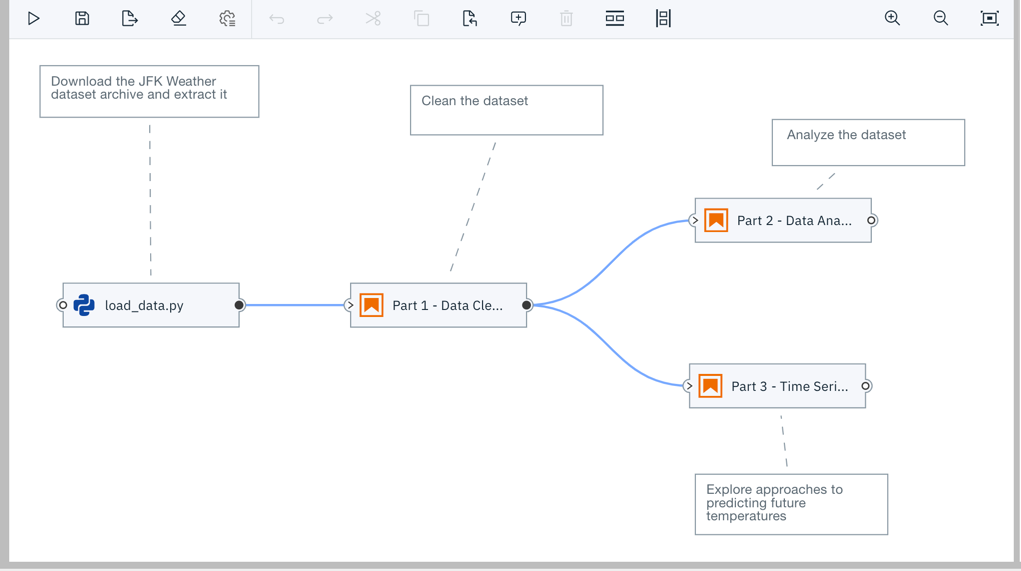
\includegraphics[scale = 0.45]{images/pipeline-in-editor.png}
\label{filtro1}
\caption{Fluxos no Elyra - JupyterLab}
\end{figure}

Para prosseguirmos com o processo de automatizaçao, foi utilizada a biblioteca Senelium do Python para acessarmos automaticamente o portal da Sinqia e baixarmos a planilha referente ao mapa de movimentos financeiros. 

Como foi preciso lidar com bastante manipulação de planilhas em XLSX e CSV, utilizamos o a biblioteca do Pandas para termos mais eficiência. 

Então, ao executarmos as tarefas por meio do Selenium, começamos as manipulações de diretórios no sistema operacional e de planilhas. 

Além das bibliotecas mencionadas, utilizamos a $Oracle_{CX}$ para nos permitir a comunicação do Python com o sistema de banco de dados, possibilitando a compilação de dados após a importação de códigos de fundos de investimentos extraídas das planilhas. Esta ação é feita por meio da inserção automática de códigos Query para o banco de dados através de documentos TXT. 






% -----------------------------------------------

\chapter{Relação Teoria de Prática}
Foi possível notar diversas relações entre a teoria explicada nas disciplinas e a prática utilizada. Fazendo a relação da teoria e prática, vários conceitos puderam ser utilizados e foram de essencial importância para o desenvolvimento das aplicações no projeto, como exemplo, as disciplinas:
Programação 1, Programação 2, Introdução à Economia para Engenheiros e Inteligência Computacional Aplicada foram as que mais contribuíram nesse estágio, embora uma delas tenha sido necessário cancelar ao longo do semestre, o que não invalida o conhecimento obtido na mesma. Como a ementa das disciplinas
são limitadas, foi necessário aprender outros conceitos e tecnologias para desenvolver os trabalhos, como por exemplo, Banco de Dados.

% -----------------------------------------------

\chapter{Dificuldades e prolemas observados}
Foram encontradas dificuldades em conciliar as atividades do estágio com as atividades
do curso, pois ocorreu no último semestre letivo de 2021 e perdurou até o início do segundo semestre de 2022, junto com uma carga horária mais complexa.
Outro fator é o trabalho Home Office (escritório em casa), por mais que tivessem as
reuniões diárias por meio de vídeo conferência, ainda não eram suficiente para o
compartilhamento das informações sobre as tecnologias e linguagens solicitadas pela empresa para o desevolvimento do projeto, bem como, o rigoroso sigilo quanto às tecnologias da
empresa que impediram de sanar dúvidas com outras pessoas.



% -----------------------------------------------

\chapter{Experiências profissionais adquiridas}

Durante o estágio, foi possível obter melhores conhecimentos de alguns ramos da
computação, principlamente no desenvolvimento de softwares e algoritmos, tendo em vista que até aquele momento não fora apresentadas durante a graduação.

Foi possível observar também que perfeiçoar os conhecimentos de programação é sempre
necessário, pois cada empresa tem seu modo de trabalhar e suas tecnologias específicas. Com
isso, pode-se realmente saber como as teorias da programação vistas nas disciplinas da grade
se aplicariam nos mais diversos ambientes de trabalhos da área.

Portanto, o estágio supervisionado foi de suma importância para auto-avaliação do que
realmente se aprendeu durante todos esses anos de graduação, proporcionando um trabalho
em equipe de forma diferente, cumprindo requisitos de um cliente real. Essa experiência
fez florescer a maturidade profissional e pessoal, e a partir da interação com um ambiente de trabalho real foi possível aperfeiçoar e aprender novas habilidades, como trabalhar em equipe e mais responsabilidade com o sigilo do projeto. 

% -----------------------------------------------

\chapter{Considerações Finais}

O estágio foi subdividido em equipes, as quais possuíam atividades diferentes, porém
estavam focadas em uma área que está em constante crescimento no mercado atualmente, o
desenvolvimento de aplicações e ferramentas para automatização de processos manuais. Por mais que a graduação tenha ensinado o que
seria basicamente necessário para atuar no mercado de trabalho, no estágio foi exigido para
realização das atividades que buscássemos conhecimento além do que foi aprendido em sala
de aula, mostrando assim a necessidade de se adaptar a determinadas situações quando
necessário, e que o ramo tecnológico sempre está se renovando, por isso sempre devemos
aprender mais.
As reuniões feitas diariamente entre os membros da equipe serviram para o
desenvolvimento das atividades, mas também proporcionou a existência de uma boa
convivência entre as partes e uma boa comunicação para o desenvolvimento das atividades
práticas, aperfeiçoando a habilidade de trabalho em equipe.



\begin{figure}[H]
\centering
\includegraphics[scale = 0.45]{images/ass_marco.png}
\label{filtro1}
\end{figure}

\centering
\>\ \>\ \textbf{Assinatura do gestor
}

% -----------------------------------------------
% Elementos pós-textuais
% -----------------------------------------------
\postextual

% -----------------------------------------------
% Referências bibliográficas
% -----------------------------------------------
\nocite{araujo:2016:abntex2}
\nocite{marcos:site}
\bibliography{referencias}




% -----------------------------------------------
% Anexos
% -----------------------------------------------
\anexos\partanexos

\chapter{Declaração de Horas Estagiadas}

\includepdf[pages=-]{anexos/declaracao_de_horas_estagio_Paloma_1621595}

\chapter{Termo de Compromisso}

\includepdf[pages=-]{anexos/CONTRATO}
\includepdf[pages=-]{anexos/termo-aditivo}

\chapter{Plano de Trabalho}

\includepdf[pages=-]{anexos/form_estagio}

\end{document}
